% ------------------------------------------------------------
% LaTeX Template für die DHBW zum Schnellstart!
% Original: https://github.wdf.sap.corp/vtgermany/LaTeX-Template-DHBW
% ------------------------------------------------------------
% ---- Präambel mit Angaben zum Dokument
\documentclass[
	fontsize=12pt,           % Leitlinien sprechen von Schriftgröße 12.
	paper=A4,
	twoside=false,
	listof=totoc,            % Tabellen- und Abbildungsverzeichnis ins Inhaltsverzeichnis
	bibliography=totoc,      % Literaturverzeichnis ins Inhaltsverzeichnis aufnehmen
	titlepage,               % Titlepage-Umgebung anstatt \maketitle
	headsepline,             % horizontale Linie unter Kolumnentitel
	abstract,              % Überschrift einschalten, Abstract muss in {abstract}-Umgebung stehen
]{scrreprt}                  % Verwendung von KOMA-Report
\usepackage[utf8]{inputenc}  % UTF8 Encoding einschalten
\usepackage[ngerman]{babel}  % Neue deutsche Rechtschreibung
\usepackage[T1]{fontenc}     % Ausgabe von westeuropäischen Zeichen (auch Umlaute)
\usepackage{microtype}       % Trennung von Wörtern wird besser umgesetzt
\usepackage{lmodern}         % Nicht-gerasterte Schriftarten (bei MikTeX erforderlich)
\usepackage{graphicx}        % Einbinden von Grafiken erlauben
\usepackage{wrapfig}         % Grafiken fließend im Text
\usepackage{setspace}        % Zeilenabstand \singlespacing, \onehalfspaceing, \doublespacing
\usepackage[
	%showframe,                % Ränder anzeigen lassen
	left=2.7cm, right=2.5cm,
	top=2.5cm,  bottom=2.5cm,
	includeheadfoot
]{geometry}                      % Seitenlayout einstellen
\usepackage{scrlayer-scrpage}    % Gestaltung von Fuß- und Kopfzeilen
\usepackage{acronym}             % Abkürzungen, Abkürzungsverzeichnis
\usepackage{titletoc}            % Anpassungen am Inhaltsverzeichnis
\contentsmargin{0.75cm}          % Abstand im Inhaltsverzeichnis zw. Punkt und Seitenzahl
\usepackage[                     % Klickbare Links (enth. auch "nameref", "url" Package)
  hidelinks,                     % Blende die "URL Boxen" aus.
  breaklinks=true                % Breche zu lange URLs am Zeilenende um
]{hyperref}
\usepackage[hypcap=true]{caption}% Anker Anpassung für Referenzen
\urlstyle{same}                  % Aktuelle Schrift auch für URLs
% Anpassung von autoref für Gleichungen (ergänzt runde Klammern) und Algorithm.
% Anstatt "Listing" kann auch z.B. "Code-Ausschnitt" verwendet werden. Dies sollte
% jedoch synchron gehalten werden mit \lstlistingname (siehe weiter unten).
\addto\extrasngerman{%
	\def\equationautorefname~#1\null{Gleichung~(#1)\null}
	\def\lstnumberautorefname{Zeile}
	\def\lstlistingautorefname{Listing}
	\def\algorithmautorefname{Algorithmus}
	% Damit einheitlich "Abschnitt 1.2[.3]" verwendet wird und nicht "Unterabschnitt 1.2.3"
	% \def\subsectionautorefname{Abschnitt}
}

% ---- Abstand verkleinern von der Überschrift 
\renewcommand*{\chapterheadstartvskip}{\vspace*{.5\baselineskip}}

% Hierdurch werden Schusterjungen und Hurenkinder vermieden, d.h. einzelne Wörter
% auf der nächsten Seite oder in einer einzigen Zeile.
% LaTeX kann diese dennoch erzeugen, falls das Layout ansonsten nicht umsetzbar ist.
% Diese Werte sind aber gute Startwerte.
\widowpenalty10000
\clubpenalty10000

% ---- Für das Quellenverzeichnis
\usepackage[
	backend = biber,                % Verweis auf biber
	language = auto,
	style = numeric,                % Nummerierung der Quellen mit Zahlen
	sorting = none,                 % none = Sortierung nach der Erscheinung im Dokument
	sortcites = true,               % Sortiert die Quellen innerhalb eines cite-Befehls
	block = space,                  % Extra Leerzeichen zwischen Blocks
	hyperref = true,                % Links sind klickbar auch in der Quelle
	%backref = true,                % Referenz, auf den Text an die zitierte Stelle
	bibencoding = auto,
	giveninits = true,              % Vornamen werden abgekürzt
	doi=false,                      % DOI nicht anzeigen
	isbn=false,                     % ISBN nicht anzeigen
    alldates=short                  % Datum immer als DD.MM.YYYY anzeigen
]{biblatex}
\addbibresource{Inhalt/literatur.bib}
\setcounter{biburlnumpenalty}{3000}     % Umbruchgrenze für Zahlen
\setcounter{biburlucpenalty}{6000}      % Umbruchgrenze für Großbuchstaben
\setcounter{biburllcpenalty}{9000}      % Umbruchgrenze für Kleinbuchstaben
\DeclareNameAlias{default}{family-given}  % Nachname vor dem Vornamen
\AtBeginBibliography{\renewcommand{\multinamedelim}{\addslash\space
}\renewcommand{\finalnamedelim}{\multinamedelim}}  % Schrägstrich zwischen den Autorennamen
\DefineBibliographyStrings{german}{
  urlseen = {Einsichtnahme:},                      % Ändern des Titels von "besucht am"
}
\usepackage[babel,german=quotes]{csquotes}         % Deutsche Anführungszeichen + Zitate


% ---- Für Mathevorlage
\usepackage{amsmath}    % Erweiterung vom Mathe-Satz
\usepackage{amssymb}    % Lädt amsfonts und weitere Symbole
\usepackage{MnSymbol}   % Für Symbole, die in amssymb nicht enthalten sind.


% ---- Für Quellcodevorlage
\usepackage{scrhack}                    % Hack zur Verw. von listings in KOMA-Script
\usepackage{listings}                   % Darstellung von Quellcode
\usepackage{xcolor}                     % Einfache Verwendung von Farben
% -- Eigene Farben für den Quellcode
\definecolor{JavaLila}{rgb}{0.4,0.1,0.4}
\definecolor{JavaGruen}{rgb}{0.3,0.5,0.4}
\definecolor{JavaBlau}{rgb}{0.0,0.0,1.0}
\definecolor{ABAPKeywordsBlue}{HTML}{6000ff}
\definecolor{ABAPCommentGrey}{HTML}{808080}
\definecolor{ABAPStringGreen}{HTML}{4da619}
\definecolor{PyKeywordsBlue}{HTML}{0000AC}
\definecolor{PyCommentGrey}{HTML}{808080}
\definecolor{PyStringGreen}{HTML}{008080}
% -- Farben für ABAP CDS
\definecolor{CDSString}{HTML}{FF8C00}
\definecolor{CDSKeywords}{HTML}{6000ff}
\definecolor{CDSAnnotation}{HTML}{00BFFF}
\definecolor{CDSComment}{HTML}{808080}
\definecolor{CDSFunc}{HTML}{FF0000}

% -- Default Listing-Styles

\lstset{
	% Das Paket "listings" kann kein UTF-8. Deswegen werden hier 
	% die häufigsten Zeichen definiert (ä,ö,ü,...)
	literate=%
		{á}{{\'a}}1 {é}{{\'e}}1 {í}{{\'i}}1 {ó}{{\'o}}1 {ú}{{\'u}}1
		{Á}{{\'A}}1 {É}{{\'E}}1 {Í}{{\'I}}1 {Ó}{{\'O}}1 {Ú}{{\'U}}1
		{à}{{\`a}}1 {è}{{\`e}}1 {ì}{{\`i}}1 {ò}{{\`o}}1 {ù}{{\`u}}1
		{À}{{\`A}}1 {È}{{\'E}}1 {Ì}{{\`I}}1 {Ò}{{\`O}}1 {Ù}{{\`U}}1
		{ä}{{\"a}}1 {ë}{{\"e}}1 {ï}{{\"i}}1 {ö}{{\"o}}1 {ü}{{\"u}}1
		{Ä}{{\"A}}1 {Ë}{{\"E}}1 {Ï}{{\"I}}1 {Ö}{{\"O}}1 {Ü}{{\"U}}1
		{â}{{\^a}}1 {ê}{{\^e}}1 {î}{{\^i}}1 {ô}{{\^o}}1 {û}{{\^u}}1
		{Â}{{\^A}}1 {Ê}{{\^E}}1 {Î}{{\^I}}1 {Ô}{{\^O}}1 {Û}{{\^U}}1
		{œ}{{\oe}}1 {Œ}{{\OE}}1 {æ}{{\ae}}1 {Æ}{{\AE}}1 {ß}{{\ss}}1
		{ű}{{\H{u}}}1 {Ű}{{\H{U}}}1 {ő}{{\H{o}}}1 {Ő}{{\H{O}}}1
		{ç}{{\c c}}1 {Ç}{{\c C}}1 {ø}{{\o}}1 {å}{{\r a}}1 {Å}{{\r A}}1
		{€}{{\euro}}1 {£}{{\pounds}}1 {«}{{\guillemotleft}}1
		{»}{{\guillemotright}}1 {ñ}{{\~n}}1 {Ñ}{{\~N}}1 {¿}{{?`}}1,
	breaklines=true,        % Breche lange Zeilen um 
	breakatwhitespace=true, % Wenn möglich, bei Leerzeichen umbrechen
	% Symbol für Zeilenumbruch einfügen
	prebreak=\raisebox{0ex}[0ex][0ex]{\ensuremath{\rhookswarrow}},
	postbreak=\raisebox{0ex}[0ex][0ex]{\ensuremath{\rcurvearrowse\space}},
	tabsize=4,                                 % Setze die Breite eines Tabs
	basicstyle=\ttfamily\small,                % Grundsätzlicher Schriftstyle
	columns=fixed,                             % Besseres Schriftbild
	numbers=left,                              % Nummerierung der Zeilen
	%frame=single,                             % Umrandung des Codes
	showstringspaces=false,                    % Keine Leerzeichen hervorheben
	keywordstyle=\color{blue},
	ndkeywordstyle=\bfseries\color{darkgray},
	identifierstyle=\color{black},
	commentstyle=\itshape\color{JavaGruen},   % Kommentare in eigener Farbe
	stringstyle=\color{JavaBlau},             % Strings in eigener Farbe,
	captionpos=b,                             % Bild*unter*schrift
	xleftmargin=5.0ex
}

% ---- Eigener JAVA-Style für den Quellcode
\renewcommand{\ttdefault}{pcr}               % Schriftart, welche auch fett beinhaltet
\lstdefinestyle{EigenerJavaStyle}{
	language=Java,                             % Syntax Highlighting für Java
	%frame=single,                             % Umrandung des Codes
	keywordstyle=\bfseries\color{JavaLila},    % Keywords in eigener Farbe und fett
	commentstyle=\itshape\color{JavaGruen},    % Kommentare in eigener Farbe und italic
	stringstyle=\color{JavaBlau}               % Strings in eigener Farbe
}

% ---- Eigener ABAP-Style für den Quellcode
\renewcommand{\ttdefault}{pcr}
\lstdefinestyle{EigenerABAPStyle}{
	language=[R/3 6.10]ABAP,
	morestring=[b]\|,                          % Für Pipe-Strings
	morestring=[b]\`,                          % für Backtick-Strings
	keywordstyle=\bfseries\color{ABAPKeywordsBlue},
	commentstyle=\itshape\color{ABAPCommentGrey},
	stringstyle=\color{ABAPStringGreen},
	tabsize=2,
	morekeywords={
		types,
		@data,
		as,
		lower,
		start,
		selection,
		order,
		by,
		inner,
		join,
		key,
		end,
		cast
	}
}

% ---- Eigener Python-Style für den Quellcode
\renewcommand{\ttdefault}{pcr}
\lstdefinestyle{EigenerPythonStyle}{
	language=Python,
	columns=flexible,
	keywordstyle=\bfseries\color{PyKeywordsBlue},
	commentstyle=\itshape\color{PyCommentGrey},
	stringstyle=\color{PyStringGreen}
}

%----- ABAP-CDS-View language
\lstdefinelanguage{ABAPCDS}{
	sensitive=false,
	%Keywords
	morekeywords={define,
		view,
		as,
		select,
		from,
		inner,
		join,
		on,
		key,
		case,
		when,
		then,
		else,
		end,
		true,
		false,
		cast,
		where,
		and,
		distinct,
		group,
		by,
		having,
		min,
		sum,
		max,
		count,
		avg
	},
	%Methoden
	morekeywords=[2]{
		div,
		currency\_conversion,
		dats\_days\_between,
		concat\_with\_space,
		dats\_add_days,
		dats\_is\_valid,
		dats\_add\_months,
		unit\_conversion,
		division,
		mod,
		abs,
		floor,
		ceil,
		round,
		concat,
		replace,
		substring,
		left,
		right,
		length
	},
	morecomment=[s][\color{CDSAnnotation}]{@}{:},
	morecomment=[l][\itshape\color{CDSComment}]{//},
	morecomment=[s][\itshape\color{CDSComment}]{/*}{*/},
	morestring=[b][\color{CDSString}]',
	keywordstyle=\bfseries\color{CDSKeywords},
	keywordstyle=[2]\color{CDSFunc}
}

  % Weitere Details sind ausgelagert

\usepackage{algorithm}                  % Für Algorithmen-Umgebung (ähnlich wie lstlistings Umgebung)
\usepackage{algpseudocode}              % Für Pseudocode. Füge "[noend]" hinzu, wenn du kein "endif",
                                        % etc. haben willst.

\makeatletter                           % Sorgt dafür, dass man @ in Namen verwenden kann.
                                        % Ansonsten gibt es in der nächsten Zeile einen Compilefehler.
\renewcommand{\ALG@name}{Algorithmus}   % Umbenennen von "Algorithm" im Header der Listings.
\makeatother                            % Zeichen wieder zurücksetzen
\renewcommand{\lstlistingname}{Listing} % Erlaubt das Umbenennen von "Listing" in anderen Titel.

% ---- Tabellen
\usepackage{booktabs}  % Für schönere Tabellen. Enthält neue Befehle wie \midrule
\usepackage{multirow}  % Mehrzeilige Tabellen
\usepackage{siunitx}   % Für SI Einheiten und das Ausrichten Nachkommastellen
\sisetup{locale=DE, range-phrase={~bis~}, output-decimal-marker={,}} % Damit ein Komma und kein Punkt verwendet wird.
\usepackage{xfrac} % Für siunitx Option "fraction-function=\sfrac"

% ---- Für Definitionsboxen in der Einleitung
\usepackage{amsthm}                     % Liefert die Grundlagen für Theoreme
\usepackage[framemethod=tikz]{mdframed} % Boxen für die Umrandung
% ---- Definition für Highlight Boxen

% ---- Grundsätzliche Definition zum Style
\newtheoremstyle{defi}
  {\topsep}         % Abstand oben
  {\topsep}         % Abstand unten
  {\normalfont}     % Schrift des Bodys
  {0pt}             % Einschub der ersten Zeile
  {\bfseries}       % Darstellung von der Schrift in der Überschrift
  {:}               % Trennzeichen zwischen Überschrift und Body
  {.5em}            % Abstand nach dem Trennzeichen zum Body Text
  {\thmname{#3}}    % Name in eckigen Klammern
\theoremstyle{defi}

% ------ Definition zum Strich vor eines Texts
\newmdtheoremenv[
  hidealllines = true,       % Rahmen komplett ausblenden
  leftline = true,           % Linie links einschalten
  innertopmargin = 0pt,      % Abstand oben
  innerbottommargin = 4pt,   % Abstand unten
  innerrightmargin = 0pt,    % Abstand rechts
  linewidth = 3pt,           % Linienbreite
  linecolor = gray!40,       % Linienfarbe
]{defStrich}{Definition}     % Name der des formats "defStrich"

% ------ Definition zum Eck-Kasten um einen Text
\newmdtheoremenv[
  hidealllines = true,
  innertopmargin = 6pt,
  linecolor = gray!40,
  singleextra={              % Eck-Markierungen für die Definition
    \draw[line width=3pt,gray!50,line cap=rect] (O|-P) -- +(1cm,0pt);
    \draw[line width=3pt,gray!50,line cap=rect] (O|-P) -- +(0pt,-1cm);
    \draw[line width=3pt,gray!50,line cap=rect] (O-|P) -- +(-1cm,0pt);
    \draw[line width=3pt,gray!50,line cap=rect] (O-|P) -- +(0pt,1cm);
  }
]{defEckKasten}{Definition}  % Name der des formats "defEckKasten"  % Weitere Details sind ausgelagert

% ---- Für Todo Notes
\usepackage{todonotes}
\setlength {\marginparwidth }{2cm}      % Abstand für Todo Notizen

% ---- Zum Einbinden von PDF-Dokumenten
\usepackage{pdfpages}


% ---- Elektronische Version oder Gedruckte Version?
% ---- Unterschied: Die elektronische Version enthält keinen Platzhalter für die Unterschrift
\usepackage{ifthen}
\newboolean{e-Abgabe}
\setboolean{e-Abgabe}{false}    % false=gedruckte Fassung

% ---- Persönlichen Daten:
\newcommand{\titel}{Programmentwurf}
\newcommand{\titelheader}{Dart Counter}
\newcommand{\arbeit}{Dart Counter}
\newcommand{\studiengang}{Informatik}
\newcommand{\studienjahr}{2023}
\newcommand{\autor}{Robin Purschwitz}
\newcommand{\autorReverse}{Purschwitz, Robin}
\newcommand{\verfassungsort}{Karlsruhe}
\newcommand{\matrikelnr}{2415691}
\newcommand{\kurs}{TINF20B2}
\newcommand{\bearbeitungsmonat}{Mai 2023}
\newcommand{\abgabe}{25. Mai 2023}
\newcommand{\bearbeitungszeitraum}{12.12.2022 - 25.05.2023}
\newcommand{\betreuerDhbw}{Dr. Lars Briem}

% ---- Metainformation für das PDF Dokument
\hypersetup{
	pdftitle    = {\titel},
	pdfsubject  = {\titelheader},
	pdfauthor   = {\autor},
	%pdfkeywords = {Keywords angeben},
	pdfcreator  = {LaTeX},
	%pdfproducer = {in der Regel pdfTeX}
}

% ---- Definition der Kopf- und Fußzeilen
\clearpairofpagestyles                          % Löschen von LaTeX Standard
\automark[section]{chapter}                     % Füllen von section und chapter
\renewcommand*{\chaptermarkformat}{}            % Entfernt die Kapitelnummer
\renewcommand*{\sectionmarkformat}{}            % Entfernt die Sectionnummer
% Angaben [für "plain"]{für "scrheadings"}
\ihead[]{\titelheader}                          % Kopfzeile links
\chead[]{}                                      % Kopfzeile mitte
\ohead[]{\rightmark}                            % Kopfzeile rechts
\ifoot[]{}                                      % Fußzeile links
\cfoot*{\sffamily\pagemark}                     % Fußzeile mitte
\ofoot[]{}                                      % Fußzeile rechts
\KOMAoptions{
   headsepline = 0.2pt,                         % Liniendicke Kopfzeile
   footsepline = false                          % Liniendicke Fußzeile
}


% ---- Hilfreiches
\newcommand{\zB}{z.\,B. }   % "z.B." mit kleinem Leeraum dazwischen (ohne wäre nicht korrekt)
\newcommand{\dash}{d.\,h. }

\newcommand{\code}[1]{\texttt{#1}} % Ist einfacher zu schreiben als ständig \texttt und erlaubt
                                   % Änderungen im Nachhinein, wenn man z.B. Inline-Code anders stylen möchte.

% ---- Silbentrennung (falls LaTeX defaults falsch / nicht gewünscht sind)
\hyphenation{HANA}         % anstatt HA-NA
\hyphenation{Graph-Script} % anstatt GraphS-cript

% ---- Beginn des Dokuments
\begin{document}
\setlength{\parindent}{0pt}              % Keine Paragraphen Einrückung.
% Dafür haben wir den Abstand zwischen den Paragraphen.
\setcounter{secnumdepth}{2}              % Nummerierungstiefe fürs Inhaltsverzeichnis
\setcounter{tocdepth}{1}                 % Tiefe des Inhaltsverzeichnisses. Ggf. so anpassen,
% dass das Verzeichnis auf eine Seite passt.
\sffamily                                % Serifenlose Schrift verwenden.

% ---- Vorspann
% ------ Titelseite
\singlespacing
\thispagestyle{empty}
\begin{titlepage}
\enlargethispage{4cm}

\begin{figure}           % Logo vom Ausbildungsbetrieb und der DHBW
	% \vspace*{-5mm} % Sollte dein Titel zu lang werden, kannst du mit diesem "Hack" 
	%                  den Inhalt der Seite nach oben schieben.
	\hfill
	\begin{minipage}{0.49\textwidth}
		\flushright
		
\includegraphics[height=2.5cm]{Bilder/Logos/Logo_DHBW.pdf} 
	\end{minipage}
\end{figure} 
\vspace*{0.1cm}

\begin{center}
	\huge{\textbf{\titel}}\\[1.5cm]
	\Large{\textbf{\arbeit}}\\[0.5cm]
	\normalsize{im Rahmen der Prüfung zum\\[1ex] \textbf{Bachelor of Science (B.Sc.)}}\\[0.5cm]
	\Large{des Studienganges \studiengang}\\[1ex]
	\normalsize{an der Dualen Hochschule Baden-Württemberg Karlsruhe}\\[1cm]
	\normalsize{von}\\[1ex] \Large{\textbf{\autor}} \\[1cm]
	% Hinweis: Manche Dozenten möchten einen Hinweis auf den Sperrvermerk auf der Titelseite.
	% \large{{\color{red}- Sperrvermerk -}}\\[1cm]
\end{center}

\begin{center}
	\vfill
	\begin{tabular}{ll}
		Abgabedatum:                     & \abgabe \\[0.2cm]
		Bearbeitungszeitraum:            & \bearbeitungszeitraum \\[0.2cm]
		Matrikelnummer, Kurs:            & \matrikelnr , \kurs \\[0.2cm]
		Gutachter der Dualen Hochschule: & \betreuerDhbw \\[2cm]
	\end{tabular} 
\end{center}
\end{titlepage}
  % Titelseite
\newcounter{savepage}
\pagenumbering{Roman}                    % Römische Seitenzahlen
\onehalfspacing

% ------ Inhaltsverzeichnis
\singlespacing
\tableofcontents

% ------ Verzeichnisse
\renewcommand*{\chapterpagestyle}{plain}
\pagestyle{plain}
%\chapter*{Formelverzeichnis}
\addcontentsline{toc}{chapter}{Formelverzeichnis} % Hinzufügen zum Inhaltsverzeichnis 

% Definition des neuen Befehls für das Einfügen der Abkürzung der Einheit
\newcommand{\acrounit}[1]{
  \acroextra{\makebox[18mm][l]{\si[per-mode=fraction,fraction-function=\sfrac]{#1}}}
}
\begin{acronym}[dmin] % längstes Kürzel wird verw. für den Abstand zw. Kürzel u. Text

	% Alphabetisch selbst sortieren - nicht verwendete Formeln rausnehmen!
	% Allgemein: \acro{KÜRZEL}[ABKÜRZUNG]{\acrounit{SI-EINHEIT}BESCHREIBUNG}

	% \acro{A}[\ensuremath{A}]{\acrounit{mm^2}Fläche}	
	% \acro{D}[\ensuremath{D}]{\acrounit{mm}Werkstückdurchmesser}	
	% \acro{dmin}[\ensuremath{d\textsubscript{min}}]{\acrounit{mm}kleinster Schaftdurchmesser}	
	% \acro{L1}[\ensuremath{L\textsubscript{1}}]{\acrounit{mm}Länge des Werkstückes Nr. 1}	
	% \acro{Fwinkel}[]{\acrounit{Grad}Freiwinkel}	
	% \acro{Kwinkel}[]{\acrounit{Grad}Keilwinkel}

\end{acronym}

\chapter*{Abkürzungsverzeichnis}
\addcontentsline{toc}{chapter}{Abkürzungsverzeichnis} % Hinzufügen zum Inhaltsverzeichnis 

\begin{acronym}[WYSISWG] % längstes Kürzel wird verw. für den Abstand zw. Kürzel u. Text

	% Alphabetisch selbst sortieren - nicht verwendete Kürzel rausnehmen!
	% \acro{AIR}{Adobe Integrated Runtime}
	% \acro{AJAX}{Asynchronous Javascript and XML}
	% \acro{ANSI}{American National Standards Institute}
	% \acro{API}{Application Programming Interface}
	% \acro{AR}{Augmented Reality}
	% \acro{BAPI}{Business Application Programming Interface}
	% \acro{BIOS}{Basic Input Output System}
	% \acro{CDMA}{Code Division Multiple Access}
	% \acro{HTTPS}{Hypertext Transfer Protocol Secure}
	% \acro{ISBN}{Internationale Standardbuchnummer}
	% \acrodefplural{ISBN}[ISBNs]{Internationale Standardbuchnummern}
	% \acro{OLAP}{Online Analytical Processing}
	% \acro{ORDBMS}{Object-Relational DataBase Management System}
	% \acro{SDK}{Software Development Kit}
	% \acro{SEO}{Search Engine Optimization}
	% \acro{SSH}{Secure Shell}
	% \acro{UEFI}{Unified Extensible Firmware Interface}
	% \acro{USB}{Universal Serial Bus}
	% \acro{VLAN}{Virtual Local Area Network}
	% \acro{WYSISWG}{What You See Is What You Get}
	% \acro{XSL}{Extensible Stylesheet Language}
	\acro{SRP}{Single Responsibility Principle}
	\acro{OCP}{Open-Closed Principle}
	\acro{ISP}{Interface Segregation Principle}
	\acro{OCP}{Open-Closed Principle}
	\acro{DRY}{Don't Repeat Yourself}
	\acro{DDD}{Domain Driven Design}
	\acro{IDE}{Integrated Development Environment}
\end{acronym}
\listoffigures                          % Erzeugen des Abbildungsverzeichnisses 
\listoftables                           % Erzeugen des Tabellenverzeichnisses
\renewcommand{\lstlistlistingname}{Quellcodeverzeichnis}
\lstlistoflistings                      % Erzeugen des Listenverzeichnisses
\setcounter{savepage}{\value{page}}


% ---- Inhalt der Arbeit
\cleardoublepage
\pagenumbering{arabic}                  % Arabische Seitenzahlen für den Hauptteil
\setlength{\parskip}{0.5\baselineskip}  % Abstand zwischen Absätzen
\rmfamily
\renewcommand*{\chapterpagestyle}{scrheadings}
\pagestyle{scrheadings}
\onehalfspacing
\chapter{Einführung}
\section{Übersicht über die Applikation}
Dart ist ein beliebtes Geschicklichkeitsspiel, das sowohl als professioneller Sport als auch als geselliges Freizeitspiel gespielt wird. Ziel des Spiels ist es, Punkte zu sammeln, indem man Pfeile (\textit{Darts}) auf ein kreisförmiges Dartboard wirft. Ein Standard-Dartboard ist in 20 nummerierte Sektionen unterteilt, wobei jeder Bereich unterschiedliche Punktzahlen vergibt. Darüber hinaus gibt es Doppel (Double) und Dreifach (Triple Felder), die den Wert der getroffenen Sektion verdoppeln bzw. verdreifachen. Das Feld dreifache 20 (\textit{triple 20}) gibt die meisten Punkte. Es gibt verschiedene Spielvarianten, wobei 501 und 301 die bekanntesten sind. Bei diesen Varianten beginnen die Spieler mit einer festgelegten Punktzahl und müssen versuchen, ihre Punktzahl exakt auf Null zu reduzieren. Das Spiel erfordert Präzision, gute Hand-Auge-Koordination und strategisches Denken. Professionelle Dart-Turniere werden weltweit ausgetragen und ziehen Tausende von Zuschauern an. Der Dart-Counter ist eine Anwendung, die es einer Gruppe aus Spielern ermöglicht dieses Spiel zu spielen. Zwar müssen die Spieler die Darts immer noch händisch auf eine Dartscheibe werfen, jedoch können die Spieler so ihre Punkte zählen und wissen, wie viele Punkte ihnen noch zu einem Checkout fehlen. Darüber hinaus können die Spieler einen ständigen Überblick über ihren aktuellen Average (Durchschnitt) behalten und am Ende eines Legs (\zB einer Runde 501) ihre Checkout-Quote (Trefferquote) sehen. Am Ende eines Gesamten Matches, welches aus mehreren Sets bestehen, welche wiederum aus mehreren Legs bestehen, haben die Spieler die Möglichkeit, ihren Spielverlauf in einer Textdatei zu speichern.
\section{Wie startet man die Applikation}
Zum starten der Applikation wird eine Java-Laufzeitumgebung und ein JDK (Version 19) benötigt. Zusätzlich wird eine \acf{IDE} zum Ausführen der Anwendung benötigt. Mit dieser IDE kann auch die Anwendung gebaut werden, um das Ausführen ohne IDE zu ermöglichen. Gestartet werden muss die Klasse '\textit{DartCounterV2/src/main/java/de/p3lina/Main.java}'. Alle Interaktionen mit der Anwendung finden dann in dem Terminal der IDE statt, mit welcher ausschlieslich mit der Tastatur interagiert werden kann. Um ein eigentliches Match zu spielen, werden zuerst Spielinformationen, wie \zB Anzahl der Spieler, Spielernamen, Startpunktanzahl etc. benötigt. Diese können, wie bereits erwähnt mit der Tastatur spezifiziert werden.
\section{Wie testet man die Applikation}
Das Testen der Applikation erfordert die Installation von Maven. Zum Testen können die Test-Klassen, welche sich in jedem Modul (application, domain etc.) unter '\textit{src/main/test}' befinden, ausgeführt werden. Die Test-Klassen können mit der IDE ausgeführt werden. Um nicht alle Tests einzeln ausführen zu müssen, besteht auch die Möglichkeit mit dem Terminal in das Wurzelverzeichnis zu navigieren und den Befehl '\textit{mvn test}' auszuführen.
\chapter{Clean Architecture}
In diesem Kapitel steht die Clean Architecture und deren zentrale Aspekte im Fokus. Zuerst erfolgt eine Analyse der Dependency Rule, einer Schlüsselregel der Clean Architecture. Untersucht werden dabei die Auswirkungen dieser Regel auf die Softwarearchitektur, ergänzt durch positive und negative Anwendungsbeispiele.

Im Anschluss daran richtet sich der Fokus auf die Struktur der Clean Architecture, wobei die einzelnen Schichten detailliert analysiert werden. Besondere Aufmerksamkeit gilt dabei den Schichten "Domain" und "Application", deren Rolle und Bedeutung innerhalb der Clean Architecture ausführlich diskutiert werden. Diese Analysen ermöglichen ein tiefgreifendes Verständnis der Clean Architecture und ihrer praktischen Anwendung.
\section{Was ist Clean Architecture}
Die \textit{Clean Architecture}, auch bekannt als die \textit{Onion Architecture}, ist ein Software-Entwurfsprinzip, das von Robert C. Martin, entwickelt wurde. Sie zielt darauf ab, eine klare und getrennte Struktur in Software-Systemen zu schaffen, um Wartbarkeit, Testbarkeit und Flexibilität zu verbessern.

Die Clean Architecture teilt eine Anwendung in konzentrische Schichten auf, wobei jede Schicht bestimmte Arten von Aufgaben erfüllt und klar definierte Abhängigkeiten aufweist. Die Schichten, von innen nach außen, sind in der Regel wie folgt:

\begin{figure}[ht]
    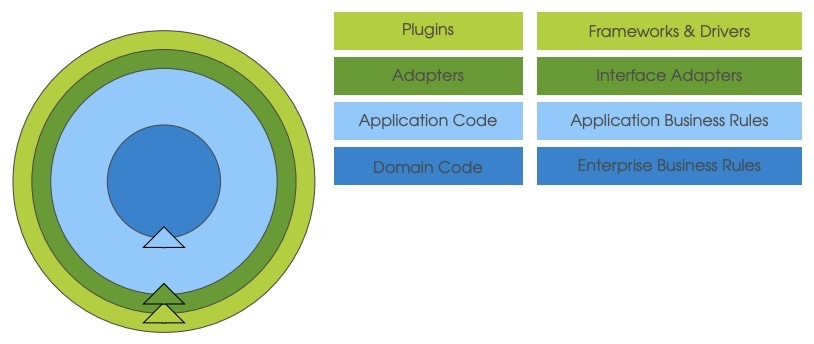
\includegraphics[width=1\textwidth]{Bilder/clean-architecture.jpeg}
    \caption{Clean Architecture Schichten}
    \label{fig:clean-architecture}
\end{figure}
\newpage
\textbf{Domain-Schicht}: Dies ist die innere Schicht, die die Geschäftslogik und die Geschäftsregeln einer Anwendung enthält. Sie hat keine Abhängigkeiten von den äußeren Schichten und repräsentiert die fundamentalen Konzepte der Anwendung, unabhängig von spezifischen technologischen Details.\\

\textbf{Anwendungs-Schicht}: Diese Schicht enthält spezifische Geschäftslogik, die sich auf bestimmte Anwendungsfälle bezieht. Sie ist von der Domain-Schicht abhängig und kann mit ihr interagieren, aber sie kennt keine Details über äußere Schichten.\\

\textbf{Adapter-Schicht}: Diese Schicht übersetzt Daten zwischen den Formaten, die für die inneren Schichten und die äußeren Schichten geeignet sind. Sie könnte beispielsweise Datenbankcode, Benutzeroberflächen-Code oder sogar Code für externe Dienste enthalten.\\

\textbf{Plugin-Schicht}: Dies ist die äußerste Schicht, die spezifische Technologien wie Datenbanken, Webserver oder Frameworks umfasst. Sie interagiert mit den inneren Schichten durch Ports und Adapter.
\newpage
Das Hauptprinzip der Clean Architecture ist die Regel der Abhängigkeitsrichtung: Abhängigkeiten sollten immer von äußeren Schichten zu inneren Schichten gerichtet sein. Dies bedeutet, dass der Code in den inneren Schichten unabhängig von spezifischen Frameworks, Datenbanken oder anderen Technologien ist, was ihn einfacher zu testen und zu warten macht.\\

Zusätzlich wird durch die klare Trennung der Verantwortlichkeiten die Einhaltung des \acf{SRP} und des \acf{OCP} aus den SOLID-Prinzipien erleichtert. Es ermöglicht auch eine bessere Modularität und Austauschbarkeit der Komponenten, da Änderungen in einer Schicht sich nicht auf die anderen Schichten auswirken sollten.

Zusammenfassend lässt sich sagen, dass die Clean Architecture ein Ansatz ist, der darauf abzielt, die Unordnung und Komplexität in Softwareprojekten zu reduzieren, indem klare Grenzen und Regeln für die Struktur und Organisation des Codes vorgegeben werden. Sie ermöglicht es Entwicklern, Systeme zu erstellen, die widerstandsfähig gegenüber technologischen Änderungen sind und die sich im Laufe der Zeit leicht anpassen und erweitern lassen.
\section{Analyse der Dependency Rule}
d
\section{Positiv-Beispiel: Dependency Rule}
\section{Negativ-Beispiel: Dependency Rule}
\section{Analyse der Schichten}
\subsection{Schicht: Domain}
\subsection{Schicht: Application}
\chapter{SOLID}
\section{Analyse Single-Responsibility-Principle (SRP)}
\subsection{Positiv Beispiel}
\subsection{Negativ Beispiel}
\section{Open Closed Principle (OCP)}
\subsection{Positiv Beispiel}
\subsection{Negativ Beispiel}
\section{Analyse Liskov-Substitution- (LSP), Interface-Segregation- (ISP), Dependency-Inversion-Principle (DIP)}
\subsection{Positiv Beispiel}
\subsection{Negativ Beispiel}
\chapter{Weitere Prinzipien}
\section{Analyse GRASP: Geringe Kopplung}
\subsection{Positiv Beispiel}
\subsection{Negativ Beispiel}
\section{Analyse GRASP: Hohe Kohäsion}
\section{Don't Repeat Yourself (DRY)}
\chapter{Unit Tests}
\section{10 Unit Tests}

\newcounter{rowcounter}
\newcommand\rownumber{\stepcounter{rowcounter}\arabic{rowcounter}}

\newcolumntype{b}{X}
\newcolumntype{s}{>{\hsize=.5\hsize}X}

\begin{table}[H]
	\centering
	\begin{tabularx}{\textwidth}{rs|b}
		& \textbf{Unit Test} & \textbf{Beschreibung} \\
		\midrule
		\rownumber & processTest:\newline HandleDartTest &
        Der Test \textit{processTest()} überprüft, ob die \textit{process()}-Methode der Klasse HandleDart die Eingabe des Benutzers korrekt verarbeitet und die erwarteten Dartpunkte zurückgibt. Der Test wird fünfmal wiederholt, um mehrere Eingaben zu simulieren und die Konsistenz der Ergebnisse zu überprüfen. \\
        \rownumber & playerDartStatusTest:\newline HandleDartTest &
        Der Test \textit{playerDartStatusTest()} überprüft, ob die Methode \textit{getDartStatus()} der Klasse \textit{HandleDart} den korrekten Dartstatus basierend auf dem aktuellen Punktestand und dem geworfenen Dart zurückgibt. Der Test verwendet verschiedene Dart-Eingaben und überprüft, ob der zurückgegebene Dartstatus den erwarteten Werten entspricht. \\
        \rownumber & getPlayerAverageOf\newline RoundTest:Player\newline AverageCalculatorTest &
        Der Test \textit{getPlayerAverageOfRoundTest()} überprüft, ob die Methode \textit{getPlayerAverageOfRound()} des \textit{PlayerAverageCalculator} die durchschnittlichen Punkte eines Spielers in einer Runde korrekt berechnet und zurückgibt. \\
        \rownumber & getPlayerAverageOf\newline LegTest:PlayerAverage\newline CalculatorTest &
        Der Test \textit{getPlayerAverageOfLegTest()} überprüft, ob die Methode \textit{getPlayerAverageOfLeg()} des \textit{PlayerAverageCalculator} die durchschnittlichen Punkte eines Spielers über alle Runden in einem \textit{Leg} korrekt berechnet und zurückgibt. \\
	\end{tabularx}
	\caption{Unit Tests 1-4}
	\label{tab:tests}
\end{table}

\begin{table}[H]
	\centering
	\begin{tabularx}{\textwidth}{rs|b}
		& \textbf{Unit Test} & \textbf{Beschreibung} \\
		\midrule
        \rownumber & getPlayersAveragesOf\newline LegTest:Player\newline AverageCalculatorTest &
        Der Test \textit{getPlayersAveragesOfLegTest()} überprüft, ob die Methode \textit{getPlayersAveragesOfLeg()} des \textit{PlayerAverageCalculator} die durchschnittlichen Punkte aller Spieler in einem \textit{Leg} als \textit{Map} zurückgibt und ob die berechneten Durchschnittswerte den erwarteten Werten entsprechen. \\
        \rownumber & getPlayerCheckoutQuote\newline OfLegTest:PlayerCheck-outQuoteCalculatorTest &
        Der Test \textit{getPlayerCheckoutQuoteOfLegTest()} überprüft, ob die Methode \textit{getPlayerCheckoutQuoteOfLeg()} des \textit{PlayerCheckoutQuoteCalculator} den Checkout-Anteil (Prozentsatz des erfolgreichen Checkouts im Vergleich zu den möglichen Checkouts) eines bestimmten Spielers in einem Leg korrekt berechnet und zurückgibt. Der Test überprüft, ob der berechnete Anteil mit dem erwarteten Wert übereinstimmt. \\
        \rownumber & getPlayersCheckoutQuote\newline OfLegTest:PlayerCheck-outQuoteCalculatorTest &
        Der Test \textit{getPlayersCheckoutQuoteOfLegTest()} prüft, ob die Methode \textit{getPlayersCheckoutQuoteOfLeg()} des \textit{PlayerCheckoutQuoteCalculator} eine Map zurückgibt, die die Checkout-Prozentsätze aller Spieler in einem Leg enthält. Der Test überprüft, ob die berechneten Anteile für jeden Spieler mit den erwarteten Werten übereinstimmen. \\
        \rownumber & getUserInputTest:\newline UserCommunication\newline ServiceTest &
        Der Test \textit{getUserInputTest()} überprüft, ob die Methode \textit{getUserInput()} des \textit{UserCommunicationService} die Benutzereingabe korrekt abruft und als \textit{UserInput}-Objekt zurückgibt. Dabei wird eine vordefinierte Zeichenkette als simulierter Benutzereingabe verwendet, und der Test vergleicht, ob die Rückgabewerte der Methode für jede Zeile der simulierten Eingabe den erwarteten Werten entsprechen. \\
	\end{tabularx}
	\caption{Unit Tests 5-8}
	\label{tab:tests}
\end{table}

\begin{table}[H]
	\centering
	\begin{tabularx}{\textwidth}{rs|b}
		& \textbf{Unit Test} & \textbf{Beschreibung} \\
		\midrule
        \rownumber & isValidDartValid\newline CaseTest:UserInputTest &
        Der Test \textit{isValidDartValidCaseTest()} überprüft, ob die Methode \textit{isValidDart()} der Klasse \textit{UserInput} den Wert \textit{true} zurückgibt, wenn die Eingabe ein gültiger Dartwert ist. In diesem Fall wird überprüft, ob \textit{SBull} als gültiger Dartwert erkannt wird. \\
        \rownumber & prepareUserDartInput\newline SBullTest:UserInputTest &
        Der Test \textit{prepareUserDartInputSBullTest()} überprüft, ob die Methode \textit{prepareUserDartInput()} der Klasse \textit{UserInput} die Benutzereingabe \textit{25} korrekt in den Dartwert \textit{SBull} umwandelt und als \textit{UserInput}-Objekt zurückgibt. Dabei wird überprüft, ob das umgewandelte Objekt den erwarteten Wert \textit{SBull} hat. \\
	\end{tabularx}
	\caption{Unit Tests 9-10}
	\label{tab:tests}
\end{table}
\section{ATRIP: Automatic}
\begin{enumerate}
    \item Einfache Ausführung: Die Unit Tests werden ausgeführt und die Ergebnisse werden in der Konsole ausgegeben.
    \item Automatisches Ablaufen: Durch die Verwendung eines global zugänglichen Scanners, kann die Systemeingabe vom Test gesetzt werden und durch den öffentlichen Scanner immer wieder weitere Zeilen aufgerunfen werden.
    \item Selbstüberprüfung: Die Unit Tests liefern durch Asserts, wie AssertEquals oder AssertTrue immer nur das Ergebnis Bestanden / Nicht Bestanden.
\end{enumerate}\newpage
\section{ATRIP: Thorough}
\textbf{Positiv Beispiel:}\\
\begin{figure}[ht]
    \centering
    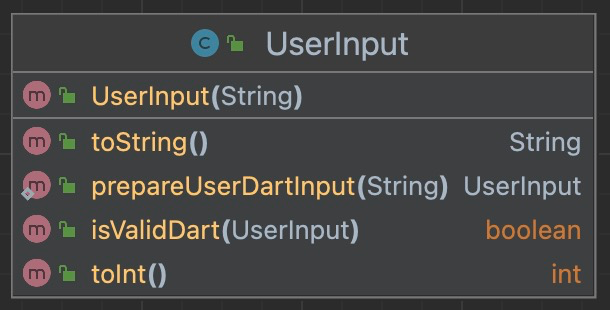
\includegraphics[width=0.8\textwidth]{Bilder/UserInputUML.png}
    \caption{UserInput UML}
    \label{fig:userinput-uml}
\end{figure}
In dieser Klasse wurden nur die Methoden \textit{isValidDart} und \textit{prepareUserDartInput} aktiv getestet. Es wurde sich dafür entschieden, da nur diese kritische und eventuell fehlerbehaftete Teile des Systems sind. Die Methoden \textit{toInt} und \textit{toString} sind hingegen kleine Hilfsmethoden, deren falsche Implementierung einen ebenso negativen Effekt auf die Anwendung hätte, jedoch sind diese Vergleichbar mit einer \textit{Getter} -und \textit{Setter}-Methode und sind somit trivial.\\
\lstinputlisting[
	label=code:userinputtest,    % Label; genutzt für Referenzen auf dieses Code-Beispiel
	caption=UserInputTest isValidDart-Methode,
	captionpos=b,               % Position, an der die Caption angezeigt wird t(op) oder b(ottom)
	style=EigenerJavaStyle,     % Eigener Style der vor dem Dokument festgelegt wurde
	firstline=1
]{Quellcode/UserInputTest.java}
Dieser Code Ausschnitt zeigt zwei Test-Methoden für die \textit{isValidDart}-Mathode. Dadurch werden beide Fälle der Methode abgedeckt: Ein gültiger Dart und ein ungültiger Dart.\\
\begin{figure}[ht]
    \centering
    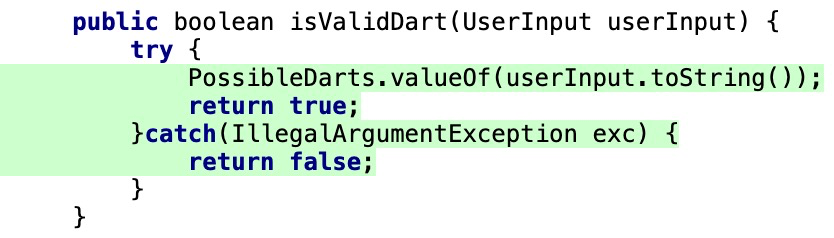
\includegraphics[width=0.8\textwidth]{Bilder/thoroughexample.png}
    \caption{vollständig abgedeckte Methode \textit{isValidDart}}
    \label{fig:isValidDart-Coverage-Code}
\end{figure}\\
Wie auf diesem Bild zu sehen ist, wurde die Methode \textit{isValidDart} vollständig abgedeckt. Dies bedeutet, dass alle möglichen Pfade der Methode durchlaufen wurden.\\\\
\textbf{Negativ Beispiel:}\\
\begin{figure}[ht]
    \centering
    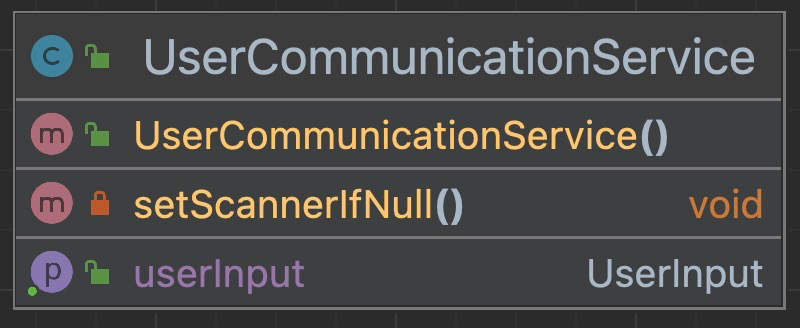
\includegraphics[width=0.8\textwidth]{Bilder/UserCommunicationServiceUML.png}
    \caption{UserCommunicationService UML}
    \label{fig:usercommunicationservice-uml}
\end{figure}
\lstinputlisting[
	label=code:usercommunicationservicetest,    % Label; genutzt für Referenzen auf dieses Code-Beispiel
	caption=UserCommunicationServiceTest Klasse,
	captionpos=b,               % Position, an der die Caption angezeigt wird t(op) oder b(ottom)
	style=EigenerJavaStyle,     % Eigener Style der vor dem Dokument festgelegt wurde
	firstline=1
]{Quellcode/UserCommunicationServiceTest.java}\newpage
\begin{figure}[ht]
    \centering
    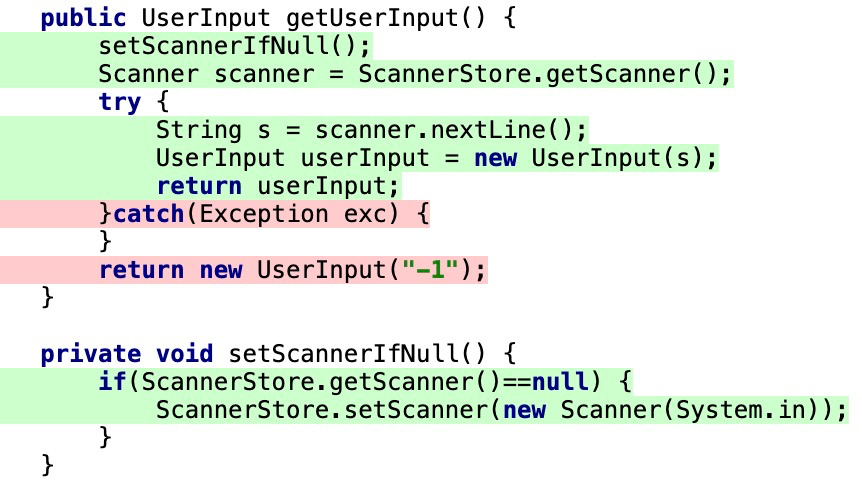
\includegraphics[width=0.8\textwidth]{Bilder/UserCommunicationService-Thorough.png}
    \caption{UserCommunicationService abgedeckter Code}
    \label{fig:usercommunicationservice-abgedeckter-code}
\end{figure}
Dieses Beispiel bezieht sich auf die Klasse \textit{UserCommunicationService}, welche für die Benutzerinteraktion verantwortlich ist. Sie verfügt über eine Methode zur Erfassung der Benutzereingaben und zur Umwandlung dieser in ein \textit{UserInput}-Objekt. Obwohl der Code innerhalb des \textit{try}-Blocks normalerweise keine Probleme verursachen sollte, muss dennoch ein Verhalten der Anwendung definiert sein, das im Fehlerfall ausgeführt werden kann. Sollte es unerwartet zu einem Fehler kommen und dieses Verhalten ausgeführt werden, würde der Test fehlschlagen und das Verhalten der Anwendung wäre unvorhersehbar. Daher erfüllt dieser Test nicht das Kriterium Thorough aus dem ATRIP-Prinzip, da er einen wesentlichen Teil des Systems, auf dem die Anwendung basiert, nicht abdeckt.
\section{ATRIP: Professional}
\textbf{Positiv Beispiel:}\\
\lstinputlisting[
	label=code:create-leg,    % Label; genutzt für Referenzen auf dieses Code-Beispiel
	caption=\textit{createLeg}-Funktion der Unit Test Klasse \textit{PlayerAverageCalculatorTest},
	captionpos=b,               % Position, an der die Caption angezeigt wird t(op) oder b(ottom)
	style=EigenerJavaStyle,     % Eigener Style der vor dem Dokument festgelegt wurde
	firstline=1
]{Quellcode/createLeg_PlayerAverageCalculatorTest.java}
In der Unit Test Klasse \textit{PlayerAverageCalculatorTest} wurde die Methode \textit{createLeg} implementiert. Diese Methode wird in der \textit{setup()}-Methode aufgerufen. Durch die Auslagerung des Codes in diese Methode, kann der Code für zukünftige Tests wiederverwendet werden.\\
\lstinputlisting[
	label=code:playerListe,    % Label; genutzt für Referenzen auf dieses Code-Beispiel
	caption=\textit{players}-Liste der Unit Test Klasse \textit{PlayerAverageCalculatorTest},
	captionpos=b,               % Position, an der die Caption angezeigt wird t(op) oder b(ottom)
	style=EigenerJavaStyle,     % Eigener Style der vor dem Dokument festgelegt wurde
	firstline=1
]{Quellcode/playersListe_PlayerAverageCalculatorTest.java}
Zuvor wurden 2 \textit{Player}-Objekte initialisiert, doch um die Erweiterbarkeit der Klasse zu verbessern wurden diese 2 Objekte in eine Liste aus Spielern gespeichert. Dadurch kann in Zukunft die Anzahl der Spieler erhöht werden, ohne dass der Code der Unit Test Klasse angepasst werden muss.\newpage
\textbf{Negativ Beispiel:}\\
\begin{figure}[ht]
    \centering
    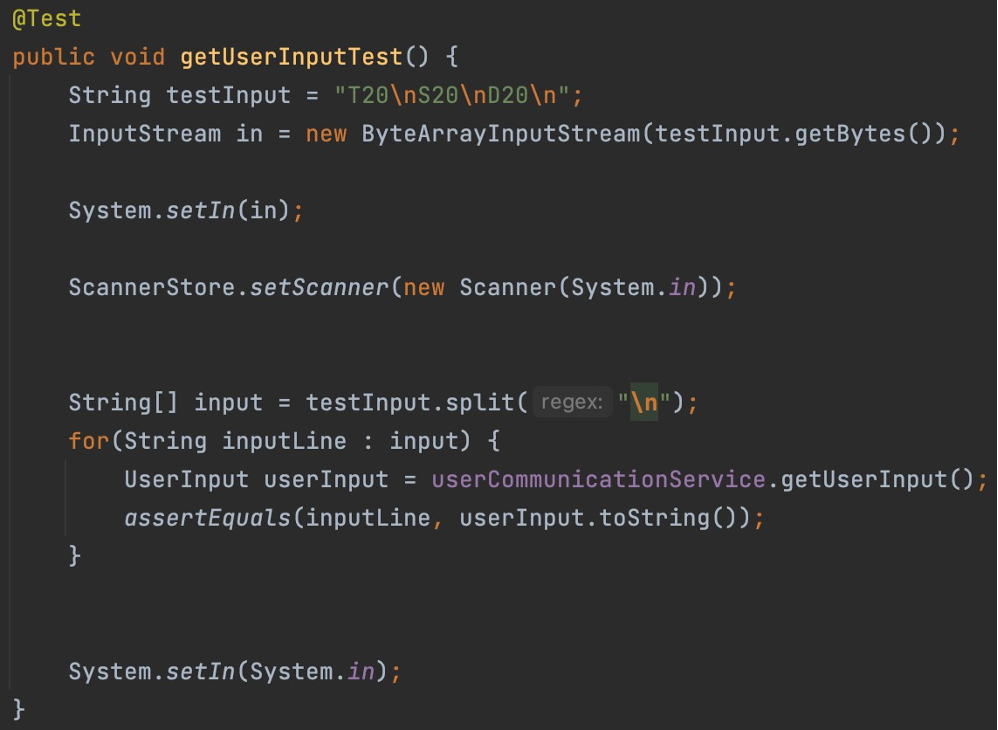
\includegraphics[width=0.8\textwidth]{Bilder/getUserInputTestCode.png}
    \caption{\textit{getUserInputTest}-Methode der Unit Test Klasse \textit{UserCommunicationServiceTest}}
    \label{fig:getUserInputTest-function}
\end{figure}\\
Als Negativ Beispiel könnte die Methode \textit{getUserInputTest} der Unit Test Klasse \textit{UserCommunicationServiceTest} dienen. Diese Methode ist für einen Entwickler, der nicht an der Entwicklung der Anwendung beteiligt war, nicht verständlich. Dies liegt daran, dass alle Operationen in einer Klasse geschehen. Durch die Einführung von Methoden, die den Code in kleinere Teile aufteilen, könnte die Lesbarkeit des Codes und die Wiederverwendbarkeit von Code-Teilen verbessert werden.\\
\section{Code Coverage}
Im Rahmen des Testens der Applikation wurde eine gezielte Vorgehensweise bei der Erstellung der Unit-Tests verfolgt. Es wurde dabei berücksichtigt, dass nicht für jede Klasse Tests notwendig sind, sondern ein Fokus auf jene gelegt wurde, die für den Verlauf der Anwendung als relevant erachtet wurden.

Die Konzentration lag insbesondere auf Klassen oder Methoden, die durch ihre Komplexität oder Wichtigkeit in der Anwendung hervorstechen. Ein Beispiel hierfür ist die Berechnung des Player-Average, welche eine komplexere Berechnung in vielen Teilen darstellt und daher explizit getestet wurde.

Aus diesem Grund wurden ausschließlich Tests für die Application-Layer entwickelt, da sie eine entscheidende Rolle für den Verlauf der Anwendung spielt. Die in dieser Schicht enthaltenen Klassen und Methoden haben direkte Auswirkungen auf den Anwendungsverlauf, weshalb ihre korrekte Funktion von großer Bedeutung ist.

Trotz alleinigen Testens der Application-Layer, blieb die Domain-Layer nicht unbeachtet. Viele der Klassen und Methoden dieser Schicht wurden passiv durch die Unit-Tests in der Application-Layer abgedeckt. Dies hat dazu geführt, dass die Domain-Layer eine Line-Coverage von knapp 50\% erreicht hat.

Zusammengefasst lässt sich sagen, dass durch diese Vorgehensweise eine gute und effiziente Testabdeckung erreicht wurde, die einen guten Überblick über den Zustand und die Qualität der Anwendung gibt.\newpage
\begin{figure}[ht]
    \centering
    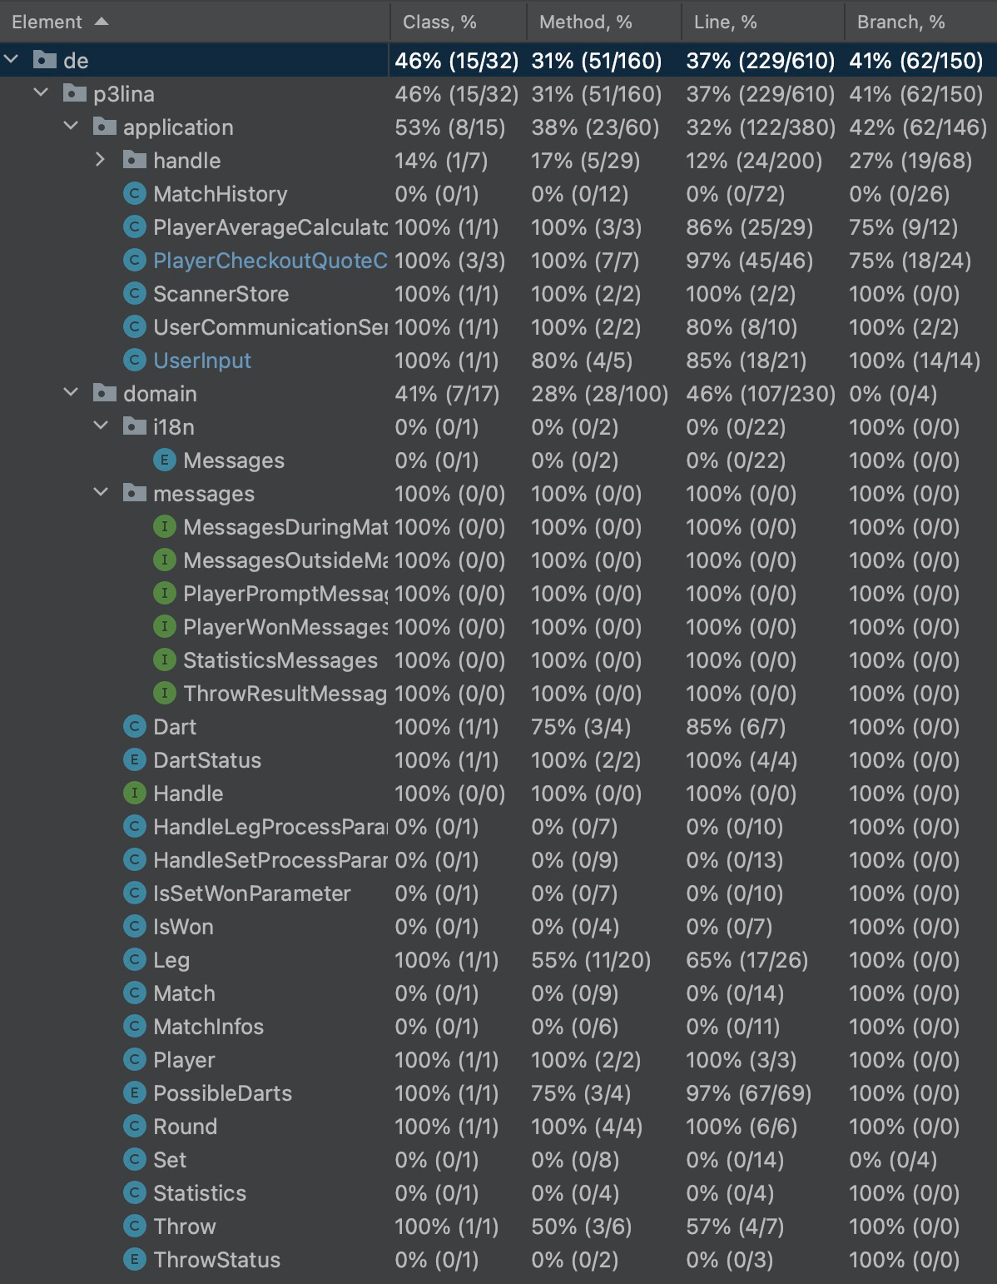
\includegraphics[width=0.7\textwidth]{Bilder/testCoverage.png}
    \caption{Überblick über die Test Coverage}
    \label{fig:test-coverage}
\end{figure}
\autoref{fig:test-coverage} gibt einen Überblick über die Abdeckung der implementierten Tests.\newpage
\section{Fakes und Mocks}
\begin{figure}[ht]
    \centering
    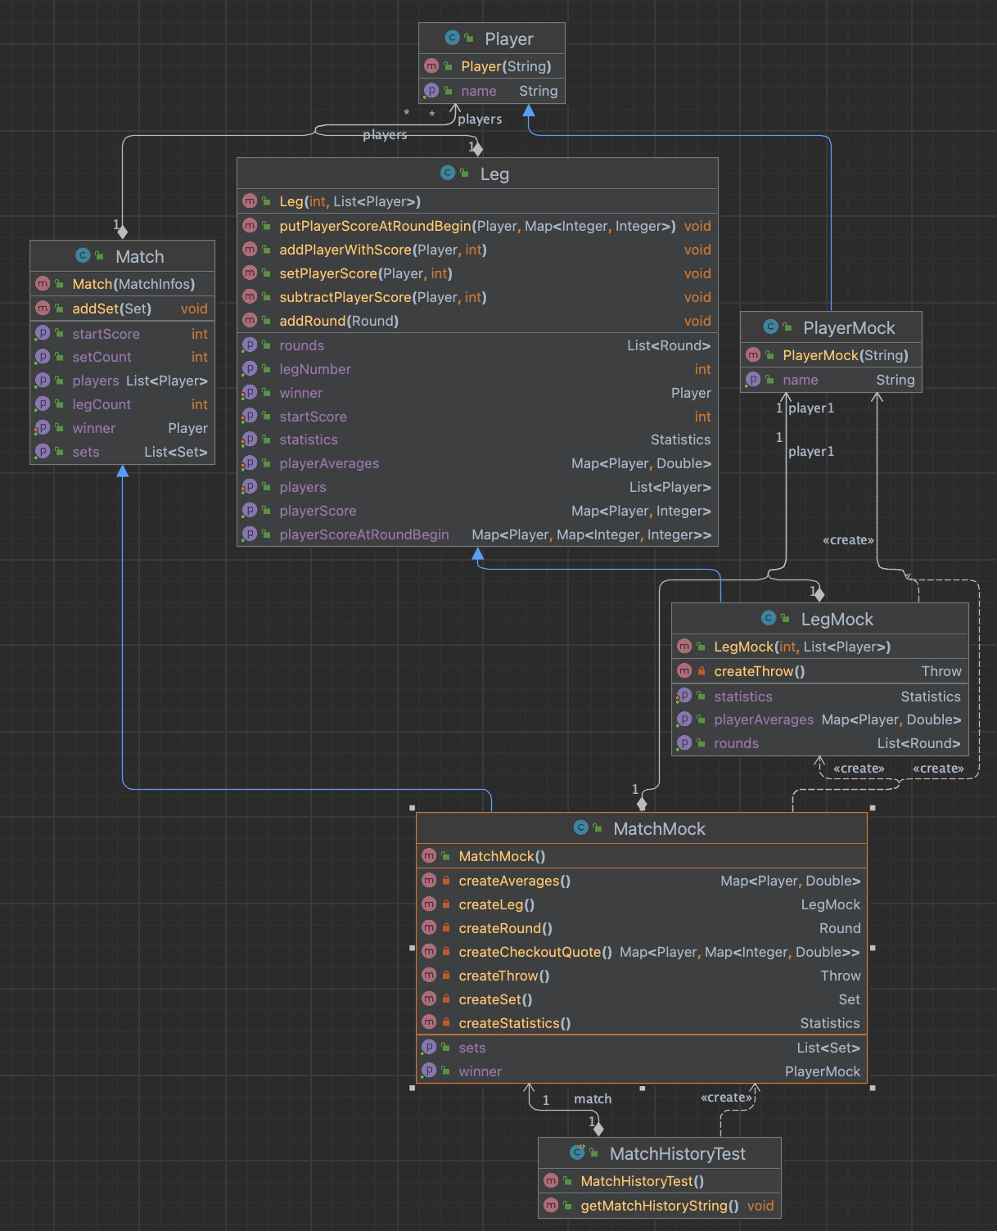
\includegraphics[width=0.8\textwidth]{Bilder/MockOverview.png}
    \caption{Übersicht der Mock-Klassen}
    \label{fig:mock}
\end{figure}
In der Unit Test Klasse \textit{MatchHistoryTest} werden zwei Fake- bzw. Mock-Objekte verwendet, um die Funktionalität der \textit{getMatchHistoryString} Methode in der MatchHistory Klasse zu testen. Die zwei Mock-Objekte, \textit{PlayerMock} und \textit{MatchMock}, simulieren das Verhalten realer Objekte innerhalb eines isolierten Testumfelds.

\textit{PlayerMock} dient dazu, das Verhalten eines \textit{Player}-Objekts zu imitieren, insbesondere im Hinblick auf die Rückgabe eines spezifischen Spielernamens. Auf der anderen Seite stellt \textit{MatchMock} ein komplexeres Szenario dar, in dem ein vollständiges Dartspiel mit Sets, Legs, Runden und Würfen simuliert wird.

Der Einsatz dieser Mock-Objekte ist wichtig, da es das Testen der getMatchHistoryString Methode ermöglicht, ohne von den tatsächlichen Implementierungen der Player und Match Klassen abhängig zu sein. Dies ist besonders nützlich, da die realen Klassen, vor allem die Match-Klasse, komplex sind.

Diese Mock-Objekte erlauben das Erstellen von vorhersehbaren Testszenarien. In diesem Fall kann garantiert werden, dass der \textit{getMatchHistoryString} Methode immer das gleiche Match mit den gleichen Spielern übergeben wird, wodurch der erwartete Ausgabestring konstant bleibt.
\chapter{Domain Driven Design}
\section{Ubiquitous}
\section{Entities}
\section{Value Objects}
\section{Repositories}
\section{Aggregates}
\chapter{Refactoring}
\section{Code Smells}
\section{2 Refactorings}
\chapter{Entwurfsmuster}
\section{Entwurfsmuster: Erbauer}
Die Erzeugung eines Match-Objektes wurde mit Hilfe eines Erbauers realisiert.
Dies ermöglichte eine erhöhte Lesbarkeit und Verständlichkeit: Durch den Einsatz des Builder-Musters wurde der Code lesbarer und einfacher zu verstehen, insbesondere da die Match-Klasse viele Parameter erwartet.
Der Einsatz ermöglichte zudem mehr Flexibilität. Bei Verwendung des Konstruktors hätten entweder separate Konstruktoren für verschiedene Kombinationen von Parametern bereitstellen oder Parameter auf einen Standardwert gesetzt werden müssen, wenn sie nicht angegeben worden wären.
Zuletzt ermöglichte der Einsatz des Erbauers eine Trennung von Erstellungslogik und Geschäftslogik. Das Builder-Muster ermöglicht es, die Erstellungslogik des eher komplexen Match-Objekts von seiner Geschäftslogik zu trennen. Das macht den Code übersichtlicher und einfacher zu warten und zu erweitern.\newpage
\begin{figure}[ht]
    \centering
    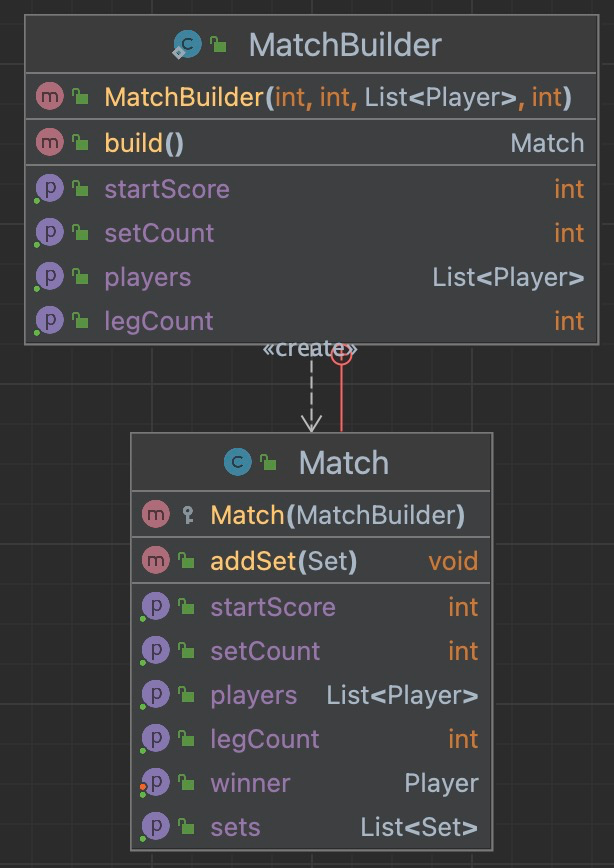
\includegraphics[width=0.5\textwidth]{Bilder/MatchBuilder.png}
    \caption{MatchBuilder}
    \label{fig:matchbuilder}
\end{figure}
\lstinputlisting[
	label=code:match-klasse,    % Label; genutzt für Referenzen auf dieses Code-Beispiel
	caption=Match-Klasse,
	captionpos=b,               % Position, an der die Caption angezeigt wird t(op) oder b(ottom)
	style=EigenerJavaStyle,     % Eigener Style der vor dem Dokument festgelegt wurde
	firstline=1
]{Quellcode/Match.java}
\section{Entwurfsmuster: Strategie}
Das Strategie-Entwurfsmuster bietet erhebliche Flexibilität, da es ermöglicht, das Verhalten von Objekten zur Laufzeit dynamisch zu ändern. Es fördert die Wiederverwendbarkeit und Austauschbarkeit von Algorithmen und erleichtert die Entkopplung von spezifischen Verhaltensweisen von den Klassen, die verwendet werden. Dadurch wird der Code sauberer und einfacher zu warten.\\
\lstinputlisting[
	label=code:handle,    % Label; genutzt für Referenzen auf dieses Code-Beispiel
	caption=Handle-Klasse,
	captionpos=b,               % Position, an der die Caption angezeigt wird t(op) oder b(ottom)
	style=EigenerJavaStyle,     % Eigener Style der vor dem Dokument festgelegt wurde
	firstline=1
]{Quellcode/Handle.java}
Umgesetzt wurde das Entwurfsmuster mit Hilfe der Handle-Klasse, die den Handle-Klassen eine Methode \textit{process} bereitstellt, die den jeweiligen Teil des Dartspiels durchlaufen lassen. Dieses Interface wird dann von allen Handle-Klassen implementiert.\\
\begin{figure}[ht]
    \centering
    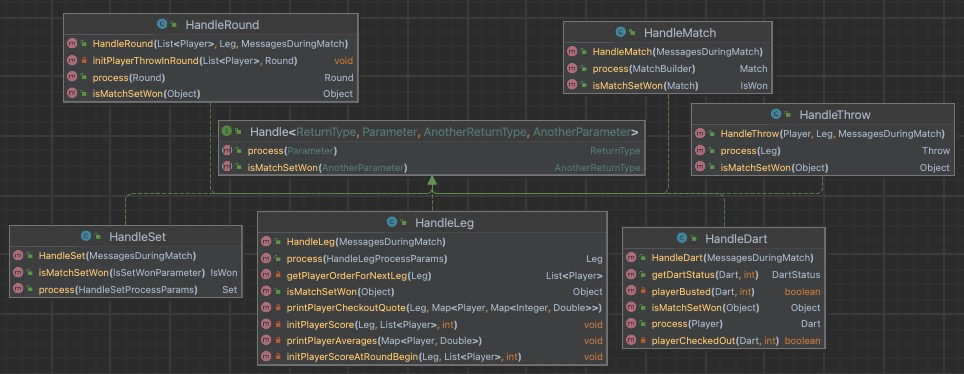
\includegraphics[width=1\textwidth]{Bilder/handleuml.png}
    \caption{Implementierung der Handle Klasse im UML}
    \label{fig:handleuml}
\end{figure}

% ---- Literaturverzeichnis
\cleardoublepage
\renewcommand*{\chapterpagestyle}{plain}
\pagestyle{plain}
\pagenumbering{Roman}                   % Römische Seitenzahlen
\setcounter{page}{\numexpr\value{savepage}+1}
\printbibliography[title=Literaturverzeichnis]

% ---- Anhang
\appendix
%\clearpage
%\pagenumbering{Roman}  % römische Seitenzahlen für Anhang

\newpage
\end{document}
